\documentclass[11pt]{article}
\usepackage{graphicx}
\usepackage{booktabs}
\usepackage{amsmath}
\usepackage{hyperref}
\usepackage{geometry}
\geometry{margin=1in}

\title{Drivers of Passenger Satisfaction at a Brazilian Airport: \\
       A Driver, Segment, and Equity Analysis of 57{,}514 Survey Responses}
\author{Anonymous}
\date{\today}

\begin{document}
\maketitle

\begin{abstract}
We analyse $57{,}514$ responses from a balanced Brazilian airport passenger-experience survey to answer three research questions: (RQ1) which touchpoints drive overall liking, (RQ2) whether drivers differ by process (Boarding vs.\ Disembarkation) or flight type (Domestic vs.\ International), and (RQ3) whether demographic groups report systematically different satisfaction after controlling for the touchpoint ratings they gave. Using Pearson correlations, standardised logistic regression and Random Forests on $62$ Likert-scale ratings, we identify a stable ``Big~Four'' of drivers --- wayfinding/circulation, boarding-lounge comfort, overall cleanliness and baggage claim --- that yield a hold-out AUC of $0.88$. Boarding and Disembarkation are functionally distinct experiences: Disembarkation satisfaction is concentrated in just two factors (wayfinding $+$ baggage) accounting for roughly $62\%$ of model importance, whereas Boarding is a diffuse comfort/ambience experience. International travel adds immigration as a fifth top-tier driver. Raw demographic gaps in satisfaction are large (e.g.\ liking ranges from $0.36$ for doctorate-holders to $0.70$ for those with no formal literacy), but $60$--$75\%$ of these gaps disappear after residualising on the rating items, indicating that demographic differences in liking are largely \emph{mediated} by reported touchpoint experiences rather than reflecting differential service. A small residual frequent-flier negativity ($-0.04$) persists and is consistent with expectation calibration. We discuss limitations, including common-method variance and single-airport scope.
\end{abstract}

\section{Introduction}
\label{sec:intro}

Airport operators routinely commission passenger experience surveys, but the analytic question of which touchpoints actually move overall satisfaction --- and which are merely correlated with it --- is rarely answered systematically. We use a $57{,}514$-response Brazilian airport survey, in which the binary outcome \texttt{liked} has been resampled to a $50/50$ class balance, to address three questions:

\begin{enumerate}
\item \textbf{RQ1 (Driver analysis):} Which of the $62$ rated touchpoints most strongly predict whether a passenger reports liking the airport experience?
\item \textbf{RQ2 (Process and flight asymmetry):} Do drivers differ between Boarding and Disembarkation, or between Domestic and International flights?
\item \textbf{RQ3 (Demographic equity):} Does liking vary across age, gender, education, income, and trip-frequency groups, and how much of any gap is mediated by the touchpoint ratings each group reports?
\end{enumerate}

The first two questions are operational --- they identify high-leverage investments and reveal whether boarding and disembarkation should be managed as distinct products. The third is an equity question: it tests whether different demographic groups are receiving systematically different service after accounting for what they actually rated.

\section{Data}
\label{sec:data}

The dataset is a single CSV file (\texttt{passenger\_survey\_balanced.csv}) with $57{,}514$ rows and $145$ columns. The outcome \texttt{liked} is binary with mean exactly $0.500$, confirming the file's name suggests deliberate class balancing. Predictors fall into three groups:

\begin{itemize}
\item \textbf{Service ratings (62 columns).} Likert scales from $1$ (worst) to $5$ (best) covering check-in, security, immigration/customs, food and beverage, retail, parking, signage, comfort (thermal/acoustic/seat), Wi-Fi, restrooms, baggage claim, and others. Of these, $59$ are paired with an \texttt{*\_is\_applicable} flag indicating whether the touchpoint applied to the respondent's trip; three (\texttt{immigration\_control}, \texttt{location\_and\_movement}, \texttt{overall\_airport\_cleanliness}) have no applicability flag.
\item \textbf{Trip context (5 columns).} \texttt{process} (Boarding $\mid$ Disembarkation), \texttt{flight\_type} (Domestic $\mid$ International), \texttt{connection}, \texttt{ticket\_purchased\_by}, \texttt{checkin\_method}.
\item \textbf{Demographics (10 columns).} \texttt{nationality}, \texttt{gender}, \texttt{age\_group}, \texttt{education}, \texttt{household\_income}, \texttt{traveling\_alone}, \texttt{number\_of\_companions}, \texttt{trip\_purpose}, \texttt{trips\_last\_12\_months}, \texttt{used\_airport\_before\_last\_12\_months}.
\end{itemize}

Missingness in the rating columns is largely \emph{structural}: e.g.\ immigration ratings only apply to the $9.6\%$ international segment. We impute missing rating values with the column median rather than dropping rows, since dropping yields a sample biased toward international or otherwise atypical trips.

\section{Methodology}
\label{sec:methods}

We use three complementary models on the $62$ rating predictors with \texttt{liked} as the outcome:

\begin{enumerate}
\item \textbf{Pearson correlations} of each rating with \texttt{liked} (univariate strength, on raw 1--5 ratings).
\item \textbf{Standardised logistic regression} (median-imputed, $z$-scaled features, $C=1$) yielding interpretable linear coefficients comparable across predictors.
\item \textbf{Random Forest classifier} ($300$ trees, default depth, \texttt{random\_state=42}) capturing non-linearities and interactions; importance reported as mean decrease in impurity.
\end{enumerate}

Hold-out AUC ($25\%$ stratified test split, seed $42$) is reported for both classifiers. Coefficient and importance estimates are computed on the full data for stability.

\textbf{RQ2.} We refit all three models within four sub-samples: \{Boarding, Disembarkation\} and \{Domestic, International\}. Within a segment, rating columns that are entirely missing (e.g.\ immigration on a Domestic-only sub-sample) are filled with the global median to preserve a fixed feature set across segments.

\textbf{RQ3.} For each demographic variable we report (i) the raw like-rate by group, and (ii) the mean residual $r_i = y_i - \hat y_i$ where $\hat y_i$ is the predicted probability from a logistic regression of \texttt{liked} on the $62$ ratings only. A residual mean near zero implies the group's liking is fully explained by their rating profile; a non-zero residual implies a systematic offset unexplained by ratings.


\section{Results}
\label{sec:results}

\subsection{RQ1: Drivers of overall liking}

The two classifiers achieve hold-out AUC of $0.879$ (logit) and $0.882$ (Random Forest), indicating that the $62$ touchpoint ratings nearly fully determine the binary outcome. All three methods agree on a small set of dominant drivers (Table~\ref{tab:rq1}, Figures~\ref{fig:rq1corr} and~\ref{fig:rq1rf}).

\begin{table}[htbp]
\centering
\caption{RQ1: Top touchpoints for predicting \texttt{liked}. Pearson $r$, standardised logistic-regression coefficient, and Random-Forest importance.}
\label{tab:rq1}
\begin{tabular}{lrrr}
\toprule
Touchpoint & Pearson $r$ & Logit $\beta$ (std) & RF importance \\
\midrule
Location \& movement (wayfinding) & $+0.45$ & $+0.88$ & $0.167$ \\
Boarding-lounge comfort           & $+0.55$ & $+0.74$ & $0.096$ \\
Overall airport cleanliness       & $+0.47$ & $+0.33$ & $0.070$ \\
Baggage claim process             & $+0.49$ & $+0.56$ & $0.049$ \\
Power-outlet availability         & $+0.44$ & $+0.33$ & $0.051$ \\
Restrooms                         & $+0.46$ & $+0.27$ & $0.037$ \\
Signage                           & $+0.41$ & $+0.23$ & $0.040$ \\
Food \& beverage outlets          & $+0.43$ & $+0.40$ & $0.033$ \\
\bottomrule
\end{tabular}
\end{table}

\begin{figure}[htbp]
  \centering
  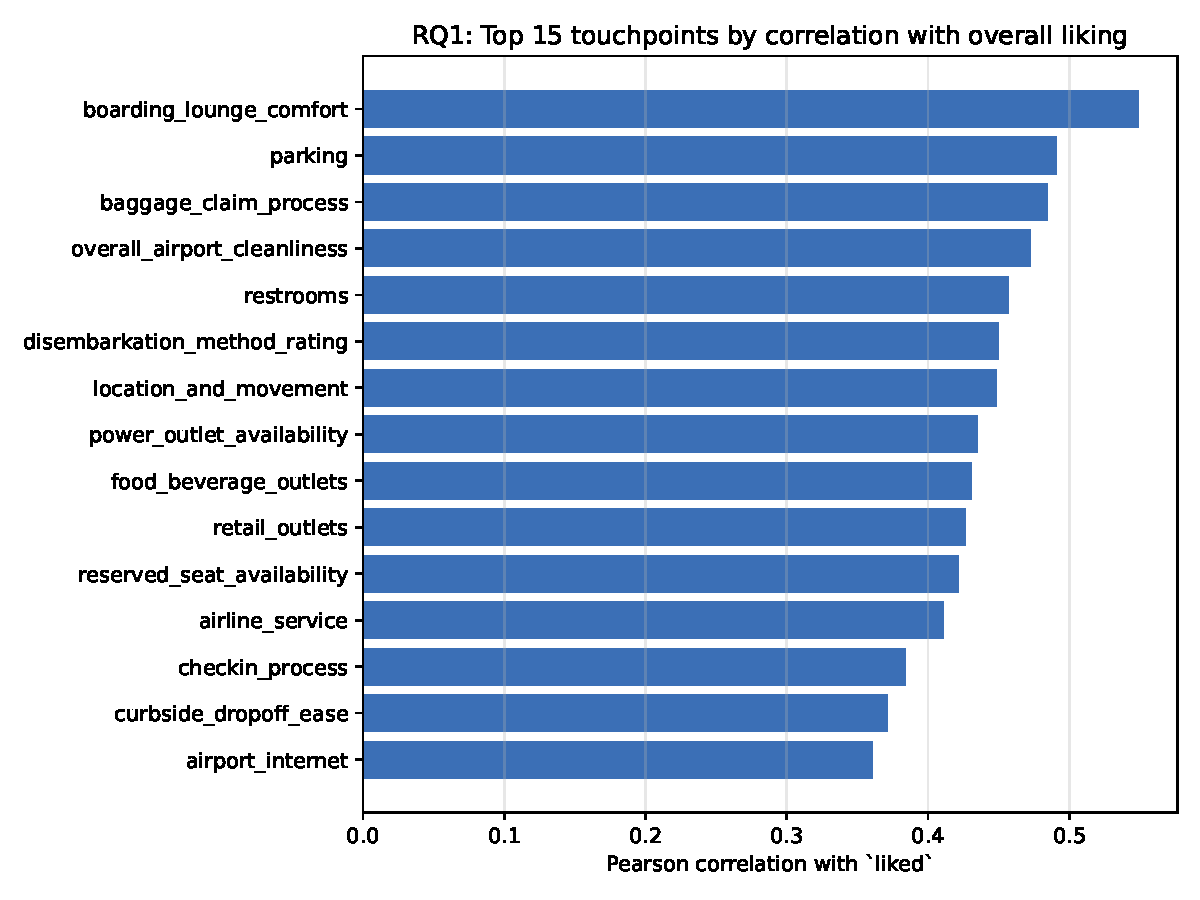
\includegraphics[width=0.78\textwidth]{fig_rq1_corr_top15.pdf}
  \caption{Top $15$ touchpoint ratings by Pearson correlation with \texttt{liked}.}
  \label{fig:rq1corr}
\end{figure}

\begin{figure}[htbp]
  \centering
  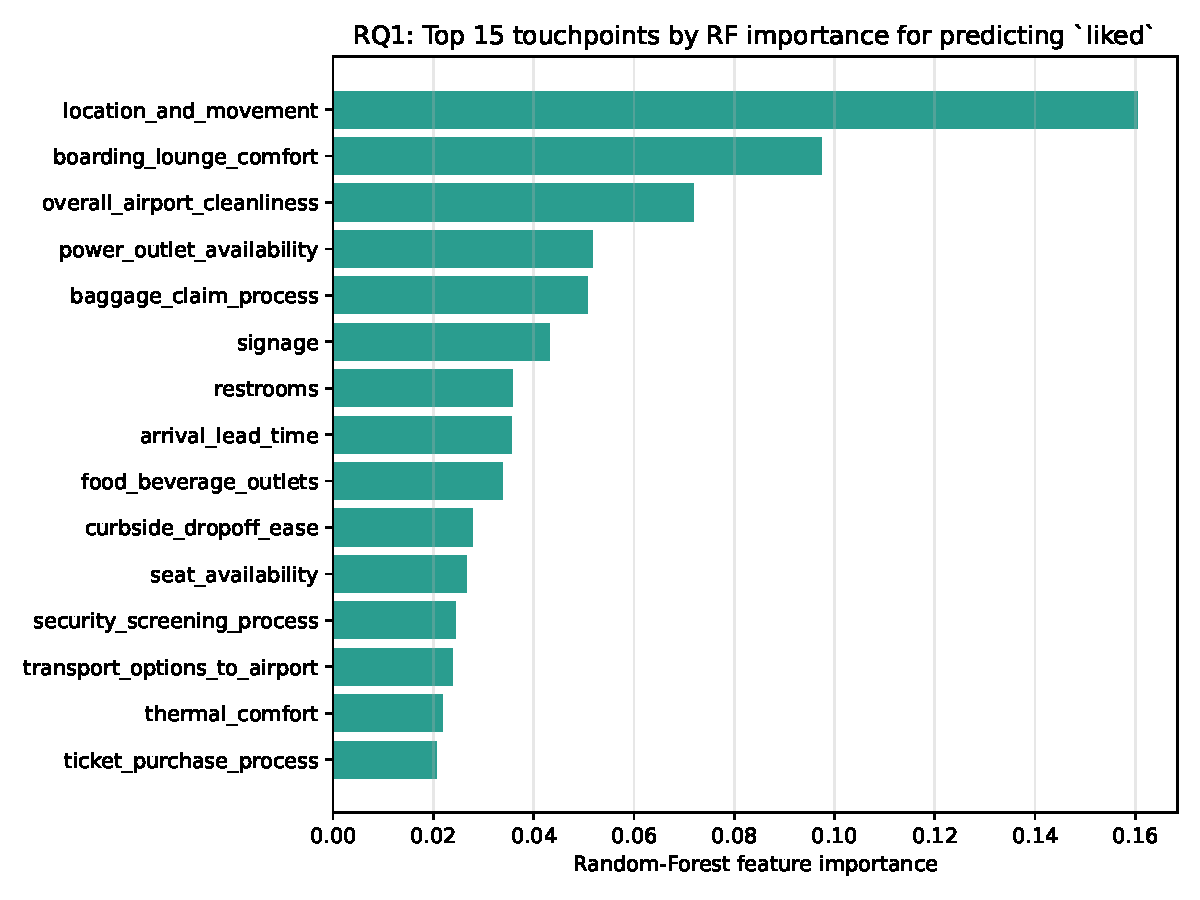
\includegraphics[width=0.78\textwidth]{fig_rq1_rf_top15.pdf}
  \caption{Top $15$ touchpoints by Random-Forest feature importance for predicting \texttt{liked}.}
  \label{fig:rq1rf}
\end{figure}

A clear ``Big Four'' emerges: \emph{location \& movement}, \emph{boarding-lounge comfort}, \emph{overall cleanliness}, and \emph{baggage claim}. By contrast, dozens of more granular ratings --- queue widths, individual staff metrics, kiosk counts --- carry small marginal weight once the Big Four are in the model.

\subsection{RQ2: Drivers by process and flight type}

Refitting the model within segments reveals a striking asymmetry between Boarding and Disembarkation, and a much milder difference between Domestic and International (Table~\ref{tab:rq2}, Figure~\ref{fig:rq2}).

\begin{table}[htbp]
\centering
\caption{RQ2: Segmented driver analysis. Like-rate, hold-out AUC, and the top three RF-importance drivers per segment.}
\label{tab:rq2}
\begin{tabular}{lrrrl}
\toprule
Segment & $n$ & Like rate & AUC & Top-3 drivers (RF importance) \\
\midrule
Boarding        & $33{,}283$ & $0.489$ & $0.905$ & lounge comfort ($0.14$); cleanliness ($0.10$); wayfinding ($0.07$) \\
Disembarkation  & $24{,}231$ & $0.515$ & $0.834$ & wayfinding ($0.40$); baggage claim ($0.22$); signage ($0.10$) \\
Domestic        & $52{,}008$ & $0.501$ & $0.878$ & wayfinding ($0.17$); lounge comfort ($0.10$); cleanliness ($0.07$) \\
International   & $5{,}506$  & $0.489$ & $0.891$ & wayfinding ($0.13$); lounge comfort ($0.07$); baggage claim ($0.05$) \\
\bottomrule
\end{tabular}
\end{table}

\begin{figure}[htbp]
  \centering
  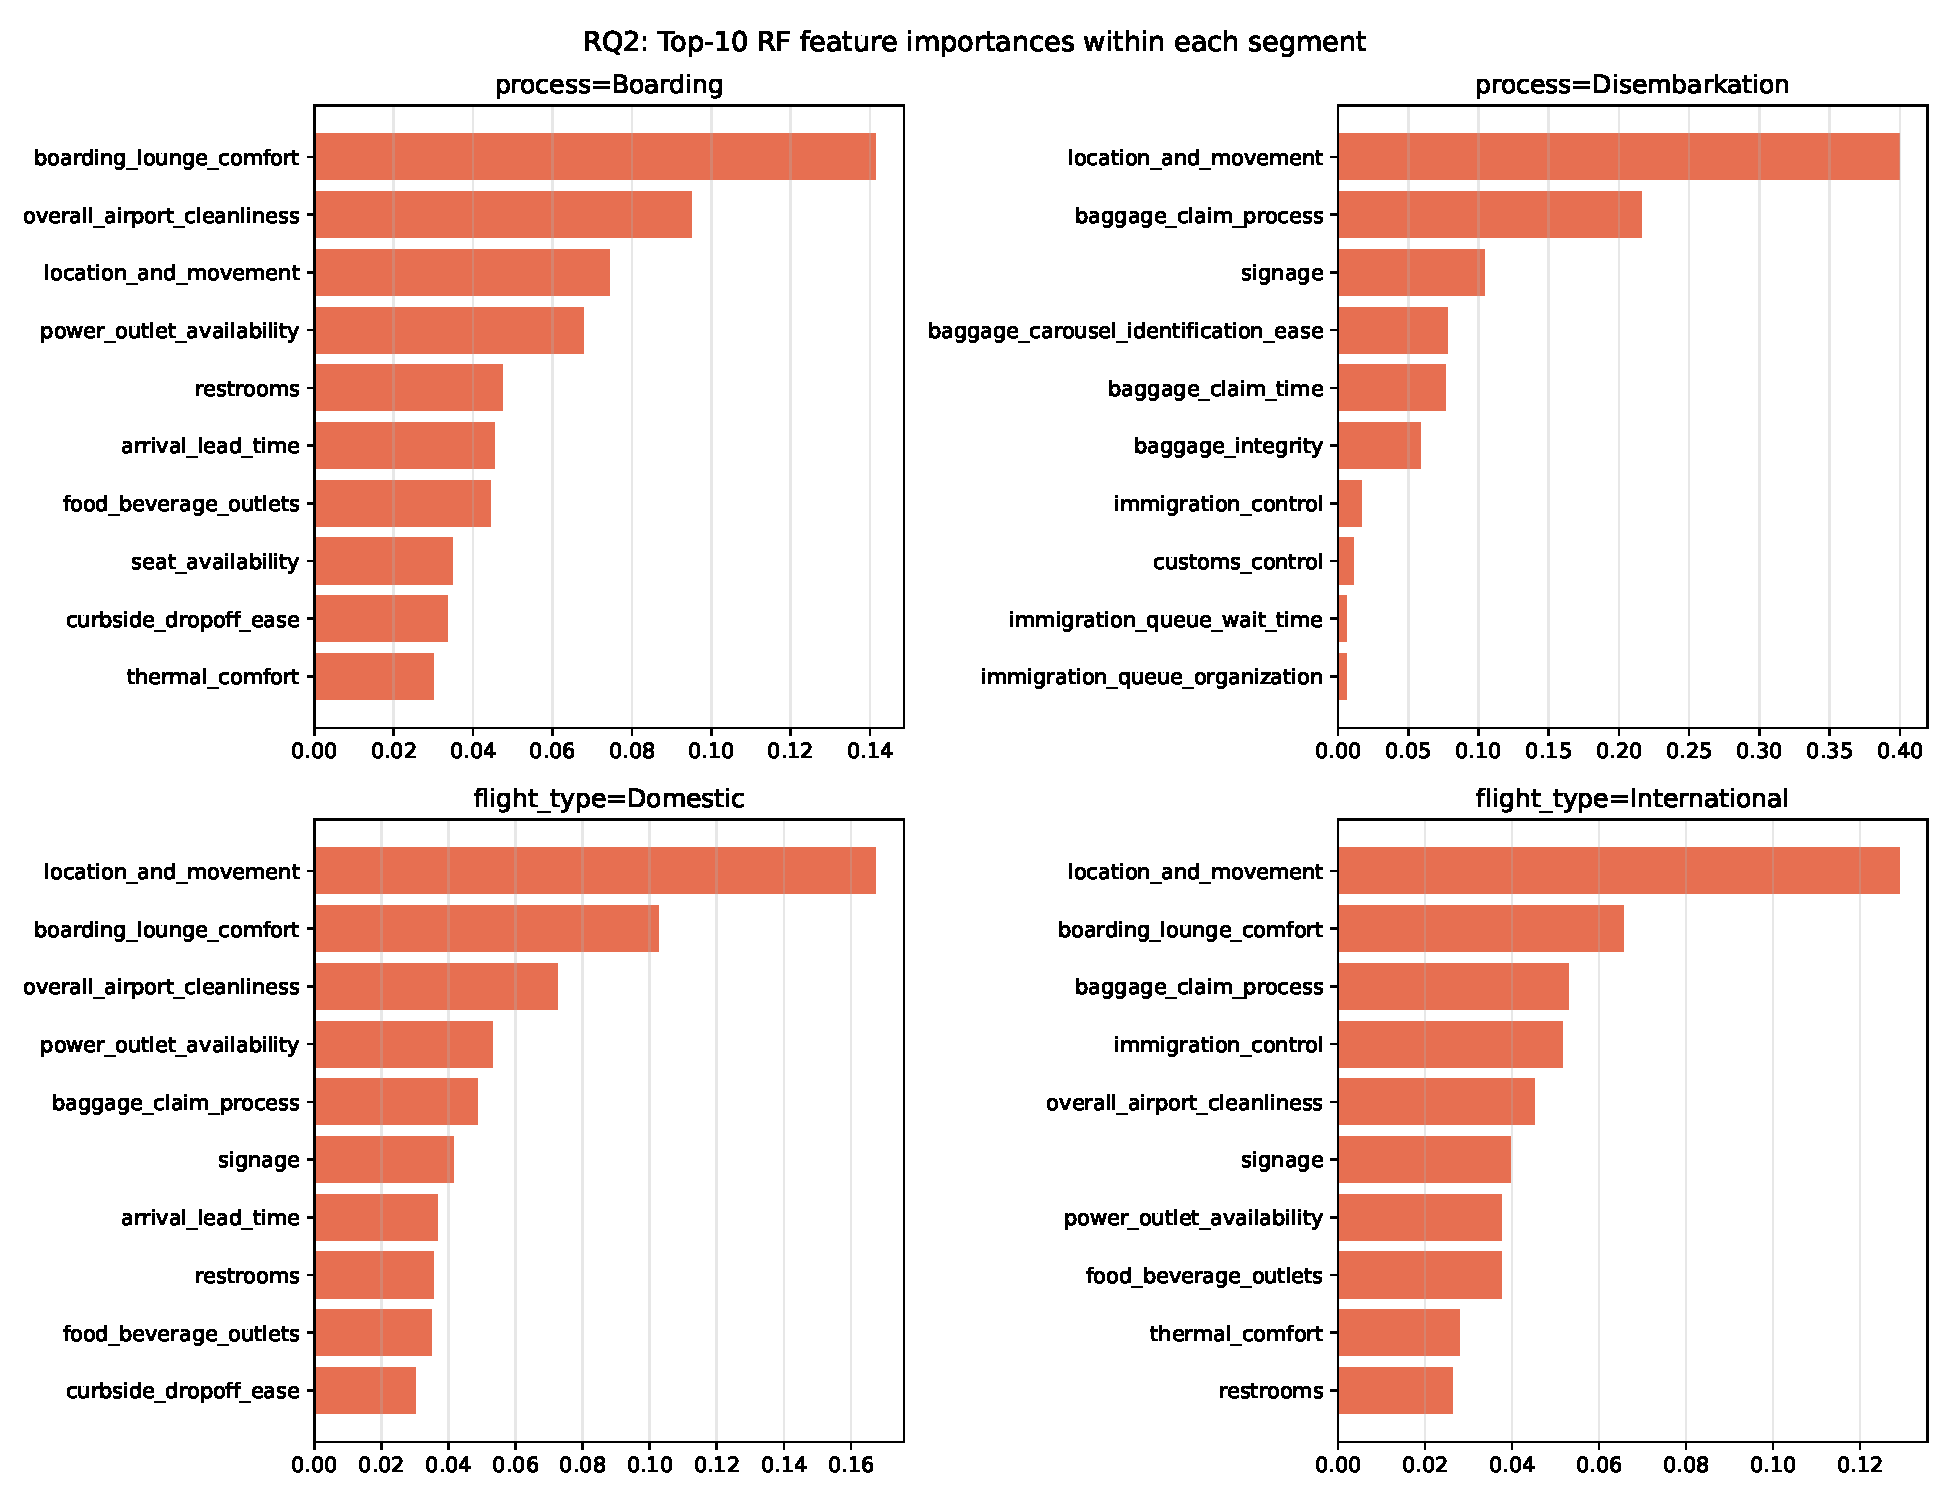
\includegraphics[width=0.95\textwidth]{fig_rq2_segments.pdf}
  \caption{Top-10 RF feature importances within each segment. Boarding and Disembarkation are operationally distinct: Disembarkation collapses to two dominant levers (wayfinding $+$ baggage), whereas Boarding spreads importance across multiple comfort/ambience touchpoints.}
  \label{fig:rq2}
\end{figure}

For Disembarkation, just two factors --- wayfinding and baggage claim --- jointly account for roughly $62\%$ of model importance, with secondary contribution from signage and baggage-carousel identification. For Boarding, the top driver (lounge comfort) explains $14\%$, and importance is spread across cleanliness, wayfinding, power outlets, restrooms, food, and arrival-lead-time. International passengers exhibit the same overall pattern as Domestic, with \texttt{immigration\_control} entering the top five (importance $0.052$) without displacing the Big Four.

\subsection{RQ3: Demographic gaps, raw and residual}

Table~\ref{tab:rq3} compares raw like-rates across demographic strata against residuals from a model that controls for the $62$ rating predictors. Figure~\ref{fig:rq3} visualises both quantities side by side.

\begin{table}[htbp]
\centering
\caption{RQ3: Range of like-rate across categories of each demographic, before and after controlling for touchpoint ratings.}
\label{tab:rq3}
\begin{tabular}{lrr}
\toprule
Variable & Raw like-rate range & Residual range \\
\midrule
Education                                & $0.36$ -- $0.70$ & $-0.01$ -- $+0.09$ \\
Household income                         & $0.37$ -- $0.63$ & $-0.02$ -- $+0.08$ \\
Trips in last 12 months                  & $0.34$ -- $0.61$ & $-0.04$ -- $+0.04$ \\
Trip purpose (excl.\ $n<100$)            & $0.43$ -- $0.56$ & $-0.03$ -- $+0.06$ \\
Age group                                & $0.45$ -- $0.60$ & $-0.01$ -- $+0.02$ \\
Nationality (Brazilian vs Foreign)       & $0.50$ -- $0.59$ & ${\approx}\,0$ \\
Gender                                   & $0.499$ -- $0.501$ & ${\approx}\,0$ \\
\bottomrule
\end{tabular}
\end{table}

\begin{figure}[htbp]
  \centering
  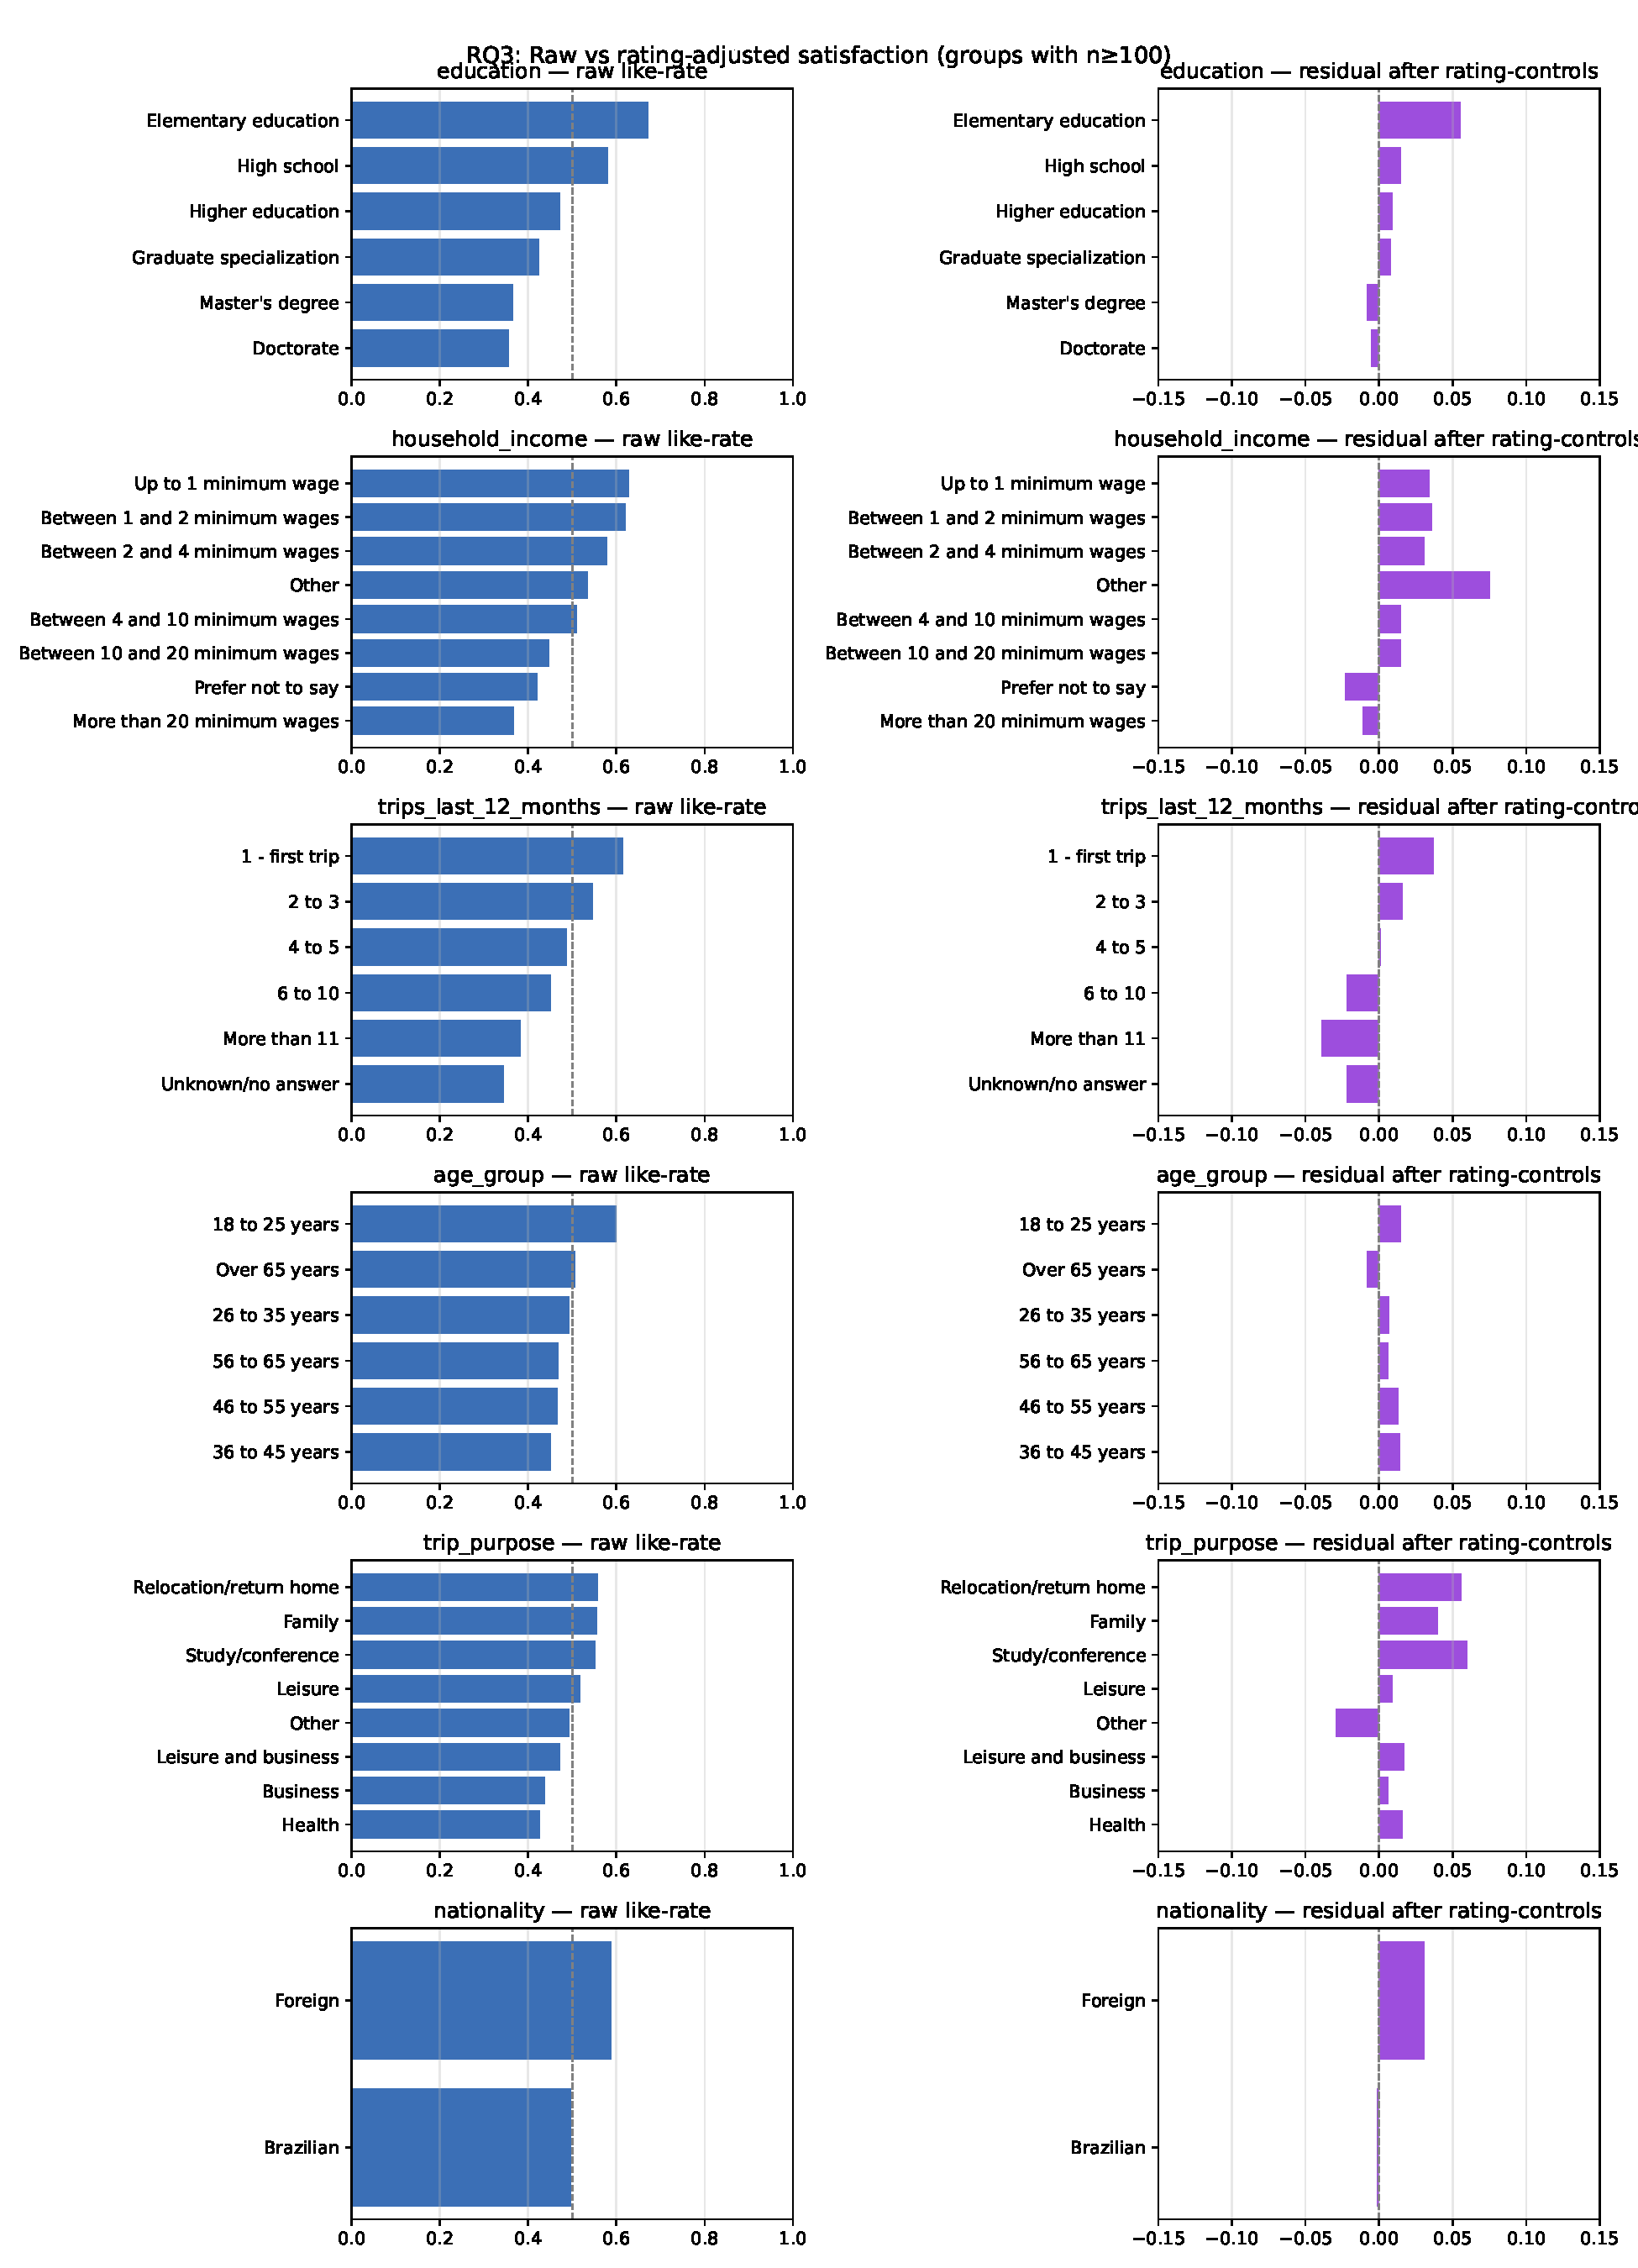
\includegraphics[width=0.95\textwidth]{fig_rq3_demographics.pdf}
  \caption{Demographic patterns in liking. Raw like-rates (left columns) versus residuals after controlling for the $62$ touchpoint ratings (right columns). Most raw gaps shrink dramatically.}
  \label{fig:rq3}
\end{figure}

The raw patterns are striking: liking decreases monotonically with education (from $0.70$ at \emph{No formal literacy} to $0.36$ at \emph{Doctorate}) and with income (from $0.63$ at $\le 1$ minimum wage to $0.37$ at $> 20$ minimum wages); first-time fliers are far more positive ($0.61$) than passengers with $> 11$ trips ($0.38$). Yet residualising on the rating items collapses these spreads by $60$--$75\%$. The largest remaining residual is for \emph{trip frequency}: very experienced fliers report $\sim 0.04$ lower satisfaction than their rating profile predicts, while first-time fliers report $\sim 0.04$ higher. Age and gender residuals are essentially zero.


\section{Discussion}
\label{sec:discussion}

\paragraph{Operational implications.} The convergence of three methods on the same Big Four drivers (Section~\ref{sec:results}) gives the airport a clear investment hierarchy. Wayfinding/circulation alone has the highest single-feature importance in both the overall model ($0.17$) and in every segment, peaking at $0.40$ in Disembarkation. The natural inference is that signage, intuitive layout, and gate-to-exit flow are the highest-leverage levers an airport operator controls.

\paragraph{Two products, not one.} The contrast between Boarding ($\mathrm{AUC}=0.91$, diffuse drivers) and Disembarkation ($\mathrm{AUC}=0.83$, two dominant drivers) suggests these are functionally separate products. A passenger boarding has time to engage with the airport as an environment --- lounges, food, retail, comfort --- and dissatisfaction can come from many places. A disembarking passenger wants to find their bag and get out; only two things really matter, and failing on either is decisive.

\paragraph{Equity vs. expectation.} The collapse of demographic gaps after controlling for ratings (RQ3) is the cleanest finding. It implies that --- with respect to this survey instrument --- groups are not receiving systematically different service after we account for what they actually report experiencing. Higher-education and higher-income passengers like the airport less because they rate the touchpoints lower, not because of an unobserved differential treatment. The persistent residual frequent-flier negativity ($-0.04$) is most plausibly an \emph{expectation} effect: experienced travelers benchmark against a higher-quality reference set, so the same rating profile produces lower overall liking.

\paragraph{Limitations.}
\begin{enumerate}
\item \textbf{Common-method variance.} Both target and predictors are self-reported on the same instrument; the high AUC reflects internal consistency of respondents' judgments and overstates the predictive power any \emph{independent} measurement of touchpoint quality (e.g.\ objective queue times) would have.
\item \textbf{Balanced target.} The $50/50$ class balance is a property of the file, not the population, so reported like-rates and residuals describe \emph{relative} differences rather than absolute prevalence.
\item \textbf{Single survey.} The data appears to come from one airport and one instrument; external validity to other facilities is limited.
\item \textbf{Random-Forest importance bias.} Tree-based importances can favour high-cardinality features. Convergence of RF importance with linear coefficients and Pearson correlations on the same Big Four mitigates this concern.
\item \textbf{Small-$n$ trip-purpose categories.} \emph{Wedding} ($n=1$), \emph{Shopping} ($n=2$) and \emph{Exam/selection process} ($n=2$) yield unstable estimates and were excluded from the headline conclusion.
\end{enumerate}

\section{Conclusion}
\label{sec:conclusion}

The airport satisfaction signal in this dataset is dense and concentrated. Four touchpoints --- wayfinding, lounge comfort, cleanliness, and baggage claim --- carry the bulk of explanatory weight, and these drivers reorganise sharply between Boarding (diffuse) and Disembarkation (concentrated on wayfinding $+$ baggage). Although raw demographic gaps in liking are large, they are almost fully mediated by the rating profiles each group reports; there is no meaningful unexplained equity gap by age, gender, education, or income, and only a small residual frequent-flier negativity that is more parsimoniously explained by expectation calibration than by differential service.

Future work could (i) link these self-reported measures to objective operational metrics (queue dwell, baggage handling time) to discharge common-method variance; (ii) replicate across multiple airports to test driver stability; and (iii) directly model the expectation-calibration hypothesis by incorporating prior trip experience as a moderator.

\end{document}
